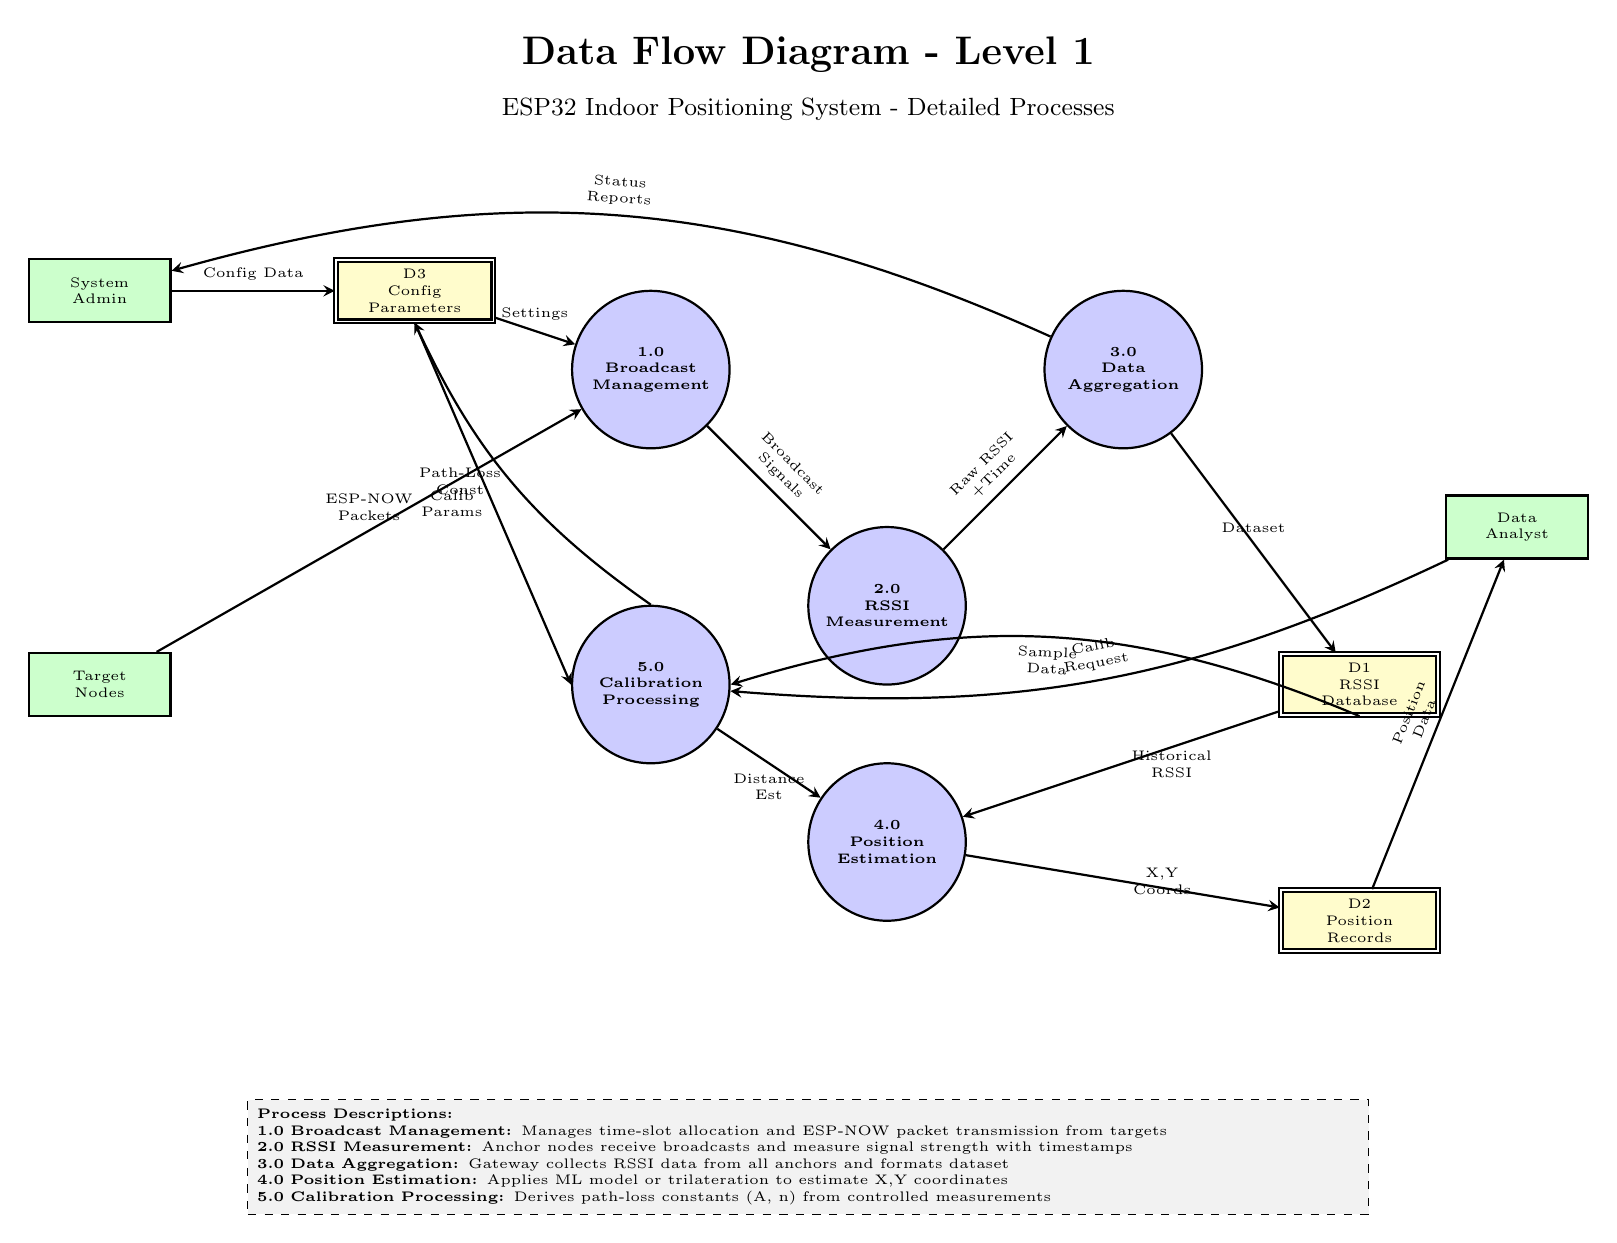
\begin{tikzpicture}[
    node distance=3cm and 4cm,
    process/.style={circle, draw, thick, minimum size=2cm, align=center, font=\tiny\bfseries, fill=blue!20},
    entity/.style={rectangle, draw, thick, minimum width=1.8cm, minimum height=0.8cm, align=center, font=\tiny, fill=green!20},
    datastore/.style={rectangle, draw, thick, minimum width=2cm, minimum height=0.6cm, align=center, font=\tiny, fill=yellow!20, double},
    flow/.style={->, thick, >=stealth},
    label/.style={font=\tiny}
]

% Title
\node[font=\Large\bfseries] at (0,9) {Data Flow Diagram - Level 1};
\node[font=\small] at (0,8.3) {ESP32 Indoor Positioning System - Detailed Processes};

% External Entities - Positioned at edges
\node[entity] (user) at (-9,6) {System\\Admin};
\node[entity] (target) at (-9,1) {Target\\Nodes};
\node[entity] (analyst) at (9,3) {Data\\Analyst};

% Data Stores - Positioned to minimize crossings
\node[datastore] (d3) at (-5,6) {D3\\Config\\Parameters};
\node[datastore] (d1) at (7,1) {D1\\RSSI\\Database};
\node[datastore] (d2) at (7,-2) {D2\\Position\\Records};

% Processes - Arranged in logical flow order
\node[process] (p1) at (-2,5) {1.0\\Broadcast\\Management};
\node[process] (p2) at (1,2) {2.0\\RSSI\\Measurement};
\node[process] (p3) at (4,5) {3.0\\Data\\Aggregation};
\node[process] (p4) at (1,-1) {4.0\\Position\\Estimation};
\node[process] (p5) at (-2,1) {5.0\\Calibration\\Processing};

% Data Flows - User/Admin to Config
\draw[flow] (user) -- node[above, label] {Config Data} (d3);
\draw[flow] (d3) -- node[above, label] {Settings} (p1);
\draw[flow] (d3.south) -- node[left, label, align=center] {Calib\\Params} (p5.west);

% Data Flows - Target to Broadcast
\draw[flow] (target) -- node[above, label, align=center] {ESP-NOW\\Packets} (p1);

% Data Flows - Main processing chain
\draw[flow] (p1) -- node[above, label, sloped, align=center] {Broadcast\\Signals} (p2);
\draw[flow] (p2) -- node[above, label, sloped, align=center] {Raw RSSI\\+Time} (p3);
\draw[flow] (p3) -- node[above, label] {Dataset} (d1);

% Data Flows - RSSI to Position Estimation
\draw[flow] (d1) -- node[right, label, align=center] {Historical\\RSSI} (p4);
\draw[flow] (p4) -- node[right, label, align=center] {X,Y\\Coords} (d2);

% Data Flows - Output to Analyst
\draw[flow] (d2) -- node[above, label, sloped, align=center] {Position\\Data} (analyst);

% Data Flows - Calibration loop
\draw[flow] (analyst) to[bend left=15] node[above, label, sloped, align=center] {Calib\\Request} (p5);
\draw[flow] (d1.south) to[bend right=20] node[below, label, sloped, align=center] {Sample\\Data} (p5.east);
\draw[flow] (p5) -- node[below, label, align=center] {Distance\\Est} (p4);
\draw[flow] (p5.north) to[bend left=15] node[left, label, align=center] {Path-Loss\\Const} (d3.south);

% Data Flows - Status feedback
\draw[flow] (p3) to[bend right=20] node[above, label, sloped, align=center] {Status\\Reports} (user);

% Legend
\node[rectangle, draw, dashed, fill=gray!10, text width=14cm, align=left, font=\tiny] at (0,-5) {
    \textbf{Process Descriptions:}\\
    \textbf{1.0 Broadcast Management:} Manages time-slot allocation and ESP-NOW packet transmission from targets\\
    \textbf{2.0 RSSI Measurement:} Anchor nodes receive broadcasts and measure signal strength with timestamps\\
    \textbf{3.0 Data Aggregation:} Gateway collects RSSI data from all anchors and formats dataset\\
    \textbf{4.0 Position Estimation:} Applies ML model or trilateration to estimate X,Y coordinates\\
    \textbf{5.0 Calibration Processing:} Derives path-loss constants (A, n) from controlled measurements
};

\end{tikzpicture}
